\documentclass[english,serif,mathserif,xcolor=pdftex,dvipsnames,table]{beamer}
\usepackage{gc3}


% \documentclass[english,serif,mathserif,usenames,dvipsnames]{beamer}
% \usetheme{gc3}

% \usepackage[T1]{fontenc}
% \usepackage[utf8]{inputenc}
% \usepackage{babel}
% \usepackage{color}

%% This is optional: it adds a few commands and environment we
%% regularly use in our slide sets


% \documentclass[english,serif,mathserif,xcolor=pdftex,dvipsnames,table]{beamer}
% \usepackage{gc3}

% \usepackage{verbatim}
% \usepackage{graphicx}
% \usepackage{alltt}
\usepackage{graphicx}

% \logo{
\includegraphics[width=\textwidth]{fig/gc3pie-logos.pdf}}

\title[GC3Pie]{%
  GC3Pie: orchestrating large scale executions of scientific applications
}
\author[Sergio Maffioletti]{%
  Sergio Maffioletti \\
  S3IT: Service and Support for ScienceIT, \\
  University of Zurich
}
\date{June.18, 2014}

\begin{document}

% title frame
\maketitle

%% quick general intro to GC3Pie 15'
%%     purpose: toolkit for building "application control logic" in Python

 % * What are the usecases we support in GC3Pie ?
 %   * High Throughput data analysis
 %   * Any sort of data processing pipelines (i.e. workflows)

 % * GC3Pie as a cloud-enabling tool (PaaS)

 % * Applications/Tasks, Collections, execution engine, backends (resource providers), sessions

%% demo of a simple use case [ with video from gbenchmark ]
%% links to documentation

% An example usecase

\begin{frame}
  \frametitle{Let's consider an example}
  \begin{block}{Cloud-based Social Network analysis}
    \begin{itemize}
    \item Quantitative {\color{Blue}empirical} research and the extended
      {\color{Blue}network analysis}.\\
    \item Challanges are the {\color{Blue}increasing size} of datasets and
      the {\color{Blue}complexity} of statistical models.
    \end{itemize}
  \end{block}
  \begin{center}
    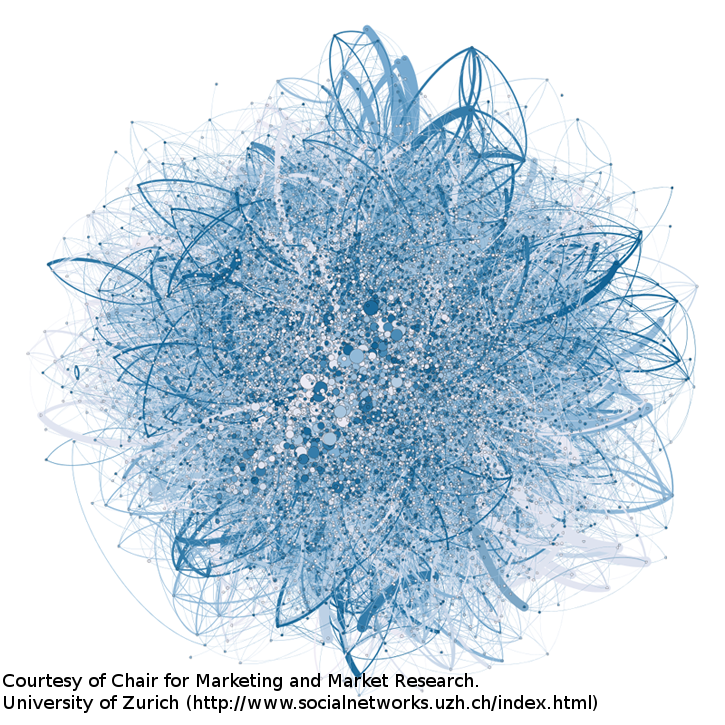
\includegraphics[width=0.4\textwidth]{fig/network.png} \\
  \end{center}
\end{frame}

\begin{frame}
  \frametitle{Scaling out from local experiment}
  \begin{itemize}
  \item User has defined an {\color{Blue}R function} that performs the statistical computations.
  \item Function is applied to  {\color{Blue}each element} of the network data.
  \item Need to process {\color{Blue}3.5M} entries.
  \item On average the function takes {\color{Blue}1-2'} to process an entry.
  \end{itemize}
\end{frame}

\begin{frame}[fragile]
  \frametitle{How S3IT did help}
\begin{lstlisting}[showstringspaces=false,basicstyle=\scriptsize\ttfamily]
...
@\HL{weight\_list}@<-apply(input.edges,
                   1,
                   GetWeight,
                   data=input.data, 
                   threads.nodes.posted=input.posted)
...
\end{lstlisting}

\end{frame}

\begin{frame}[fragile]
  \frametitle{How did GC3Pie help}

\begin{lstlisting}[showstringspaces=false,basicstyle=\tiny\ttfamily]
class GWeightApplication(Application):
    """
    Custom class to wrap the execution of the R scripts passed in src_dir.
    """
    application_name = 'gweight'

    def __init__(self, edges_data_filename, **extra_args):
        # Check consistency of input data
        # Build remote command invocation
        # e.g. Rscript --vanilla \$MASTER \$WEIGHT \$EDGES \$DATA \$THREADS
        ...

        Application.__init__(
            self,
            arguments = arguments,
            inputs = inputs,
            outputs = outputs,
            stdout = 'gweight.log',
            join=True,
            executables = ['wrapper.sh'],
            **extra_args)
\end{lstlisting}

\end{frame}

\begin{frame}[fragile]
  \frametitle{How GC3Pie did help}
\begin{lstlisting}[showstringspaces=false,basicstyle=\tiny\ttfamily]
./gweight.py -h
usage: gweight [-h] [-V] [-v] [--config-files CONFIG_FILES] [-c NUM]
               [-m GIGABYTES] [-r NAME] [-w DURATION] [-s PATH] [-u URL] [-N]
               [-C NUM] [-J NUM] [-o DIRECTORY] [-l [STATES]] [-k [NUM]]
               [-M [PATH]] [-D [PATH]] [-F [PATH]] [-T [PATH]]
               edges_data
\end{lstlisting}
Let's see how it works\dots
\end{frame}

\begin{frame}
  \begin{center}
    \huge{What is {\color{Blue} GC3Pie} and \\ why do we need something like that ?}
  \end{center}
\end{frame}

\begin{frame}
  \frametitle{Supervised execution}
  \begin{block}{}
    Need to automate the execution of a large number of different
    applications on a variety of computational resources.
  \end{block}

  \begin{enumerate}
  \item{\textbf{Access}} to computational resources
  \item{\textbf{Supervise}} execution of collection of jobs
  \item{\textbf{Handling}} of error conditions individually
  \item{\textbf{Post-process}} and store results
  \end{enumerate}
\end{frame}


\begin{frame}
  \frametitle{The issues GC3Pie wants to solve}
  \begin{enumerate}
  \item \textbf{Portability:} Cannot run on a different cluster without
    rewriting all the scripts.
  \item \textbf{Code reuse:} Scripts are often very tied to a certain purpose, so
    they are difficult to reuse.
  \item \textbf{Heavy maintenance:} the more a script does its job well, the more
    you'll find yourself adding \emph{generic} features and maintaining
    requests from other users.
  \end{enumerate}
\end{frame}


\begin{frame}
\frametitle{What is GC3Pie ?}
  \begin{block}{}
    GC3Pie is a {\color{Blue} Python} toolkit:
  \end{block}

  \begin{block}{}
    it provides the building blocks to write Python scripts to run large {\color{Blue} computational campaigns} and
  \end{block}

  \begin{block}{}
    to {\color{Blue} combine} several tasks into a dynamic
    {\color{Blue} workflow}.
  \end{block}
\end{frame}

\begin{frame}
\frametitle{What is GC3Pie ?}

  GC3Pie consists of three main components:

  \begin{block}{GC3Libs:} Python library for controlling the life-cycle of computational job collections. \end{block}
  \begin{block}{GC3Apps:} A collection of driver scripts to run large job campaigns. \end{block}
  \begin{block}{GC3Utils:} This is a small set of low-level utilities exposing the main functionality provided by GC3Libs. \end{block}
\end{frame}

%% \begin{frame}[fragile]
%%   \frametitle{An example: ggamess}
%%   \begin{alltt}
%% import gc3libs
%% from gc3libs.application.gamess
%%      {\color{Blue}import} GamessApplication
%% from gc3libs.cmdline
%%      {\color{Blue}import} SessionBasedScript

%% class {\color{Violet} GGamessScript}({\color{Violet}SessionBasedScript}):
%%   def \_\_init\_\_(self):
%%     SessionBasedScript.\_\_init\_\_(
%%        self,
%%        application = {\color{Violet}GamessApplication},
%%        input_filename_pattern = '{\color{Green}*.inp}'
%%     )

%% if \_\_name\_\_ == '{\color{Green}\_\_main\_\_}':
%%   GGamessScript().{\color{Blue}run()}
%% \end{alltt}
%% \end{frame}


%% \begin{frame}
%%   \frametitle{ggamess example}
%%   \begin{center}
%%     \large{The video...}
%%   \end{center}
%% \end{frame}

\begin{frame}
  \frametitle{GC3Pie for developers}
    \begin{block}{}
      Programming model based on customization of base classes through
      inheritance ({\color{Blue}Template method} pattern)
    \end{block}

    \begin{block}{}
      Different level of {\color{Blue}interfaces} depending on the control required
    \end{block}

    \begin{block}{}
      {\color{Blue}SessionBasedScript} is the highest level of abstraction
    \end{block}
\end{frame}

\begin{frame}
  \frametitle{How is GC3Pie different? (I)}

  \begin{block}{}
    GC3Pie runs specific \textbf{applications}, not generic jobs.
  \end{block}

   \begin{block}{}
     That is, GC3Pie exposes \texttt{Application} classes whose programming
    interface is adapted to the specific task/computation a scientific
    application performs.
  \end{block}

  \begin{block}{}
    You can add your own application by specializing the generic
    \texttt{Application} class.
  \end{block}
\end{frame}

\begin{frame}
  \frametitle{How is GC3Pie different? (II)}

  \begin{block}{}
    GC3Pie can run applications in parallel, or sequentially, or any
    combination of the two, and do arbitrary processing of data in the
    middle.
  \end{block}

  \begin{block}{}
    Think of {\color{Blue}workflows}, except you can write them in the Python
    programming language.
  \end{block}

  \begin{block}{}
    Which means, you can create them dynamically at runtime, adapting
    the schema to your problem.
  \end{block}
\end{frame}

\begin{frame}
  \frametitle{GC3Pie Execution model}
  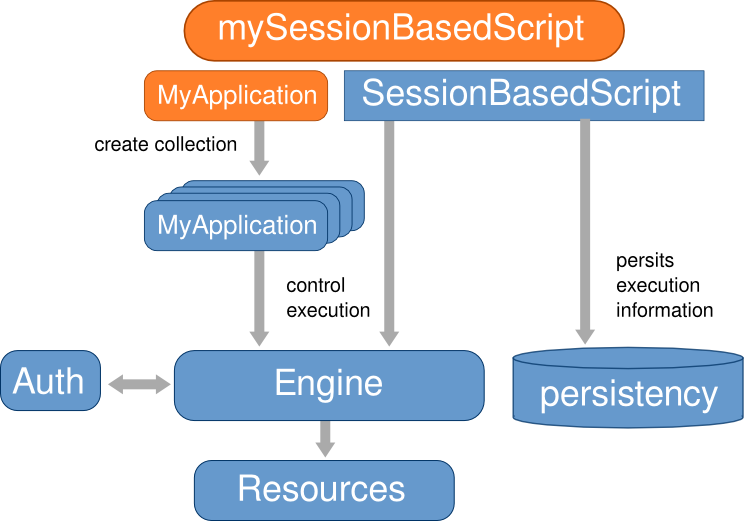
\includegraphics[width=0.8\textwidth]{fig/GC3Pie_execution_model}
\end{frame}

\begin{frame}
  \frametitle{GC3Pie Execution model}
  \begin{columns}
    \column{0.5\textwidth}
      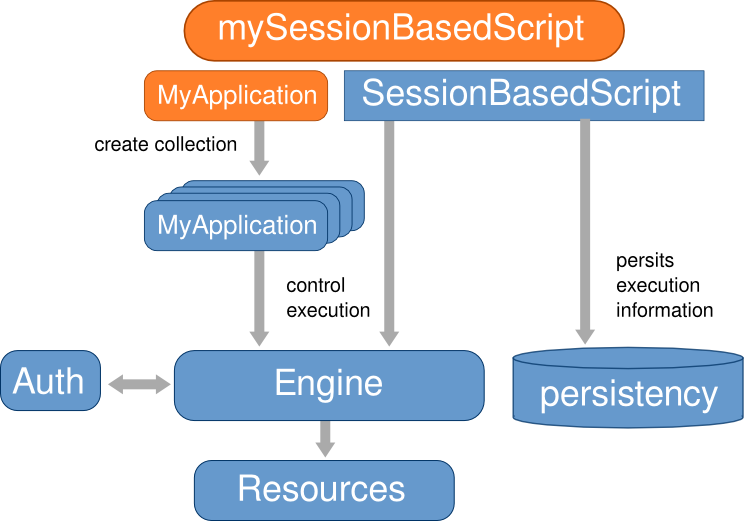
\includegraphics[width=1\textwidth]{fig/GC3Pie_execution_model}
    \column{0.6\textwidth}
  \begin{block}{}
    An application is a subclass of the \texttt{gc3libs.Application}
    class. \\
  \end{block}

  \begin{block}{}
    Applications can be grouped in {\color{Blue}collections}
  \end{block}
  \end{columns}
\end{frame}

\begin{frame}
  \frametitle{GC3Pie Execution model}
  \begin{columns}
    \column{0.5\textwidth}
      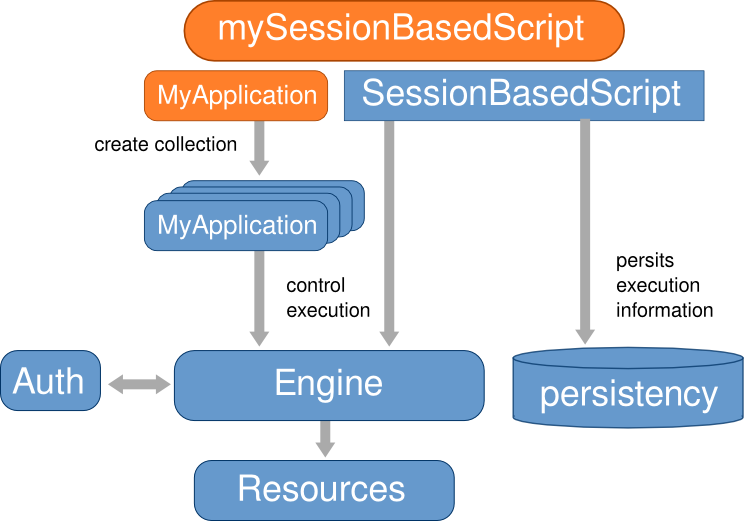
\includegraphics[width=1\textwidth]{fig/GC3Pie_execution_model}
    \column{0.6\textwidth}
  \begin{block}{}
    Execution of collections is delegated to an \texttt{Engine}.
  \end{block}

  %% \begin{block}{}
  %%   Execution Engine handles the access to computational {\color{Blue}resources}
  %%   (also verifying the proper {\color{Blue}authentication} mechanism)
  %% \end{block}
  \end{columns}
\end{frame}

\begin{frame}
  \frametitle{GC3Pie Execution model}
  \begin{block}{Resource}
    is a {\color{Blue}computational endpoint} where the
    {\color{Blue}execution} of the {\it Application} will take place.
  \end{block}
  \begin{block}{}
    GC3Pie can execute processes on a large variety of computational
    resources:
    {\color{Blue}cloud-based} VMs, {\color{Blue}batch-queueing}
    clusters, computational {\color{Blue}Grids}, and -of course- any
    Linux/UNIX host where you can {\color{Blue}SSH} into.

    %% GC3Pie supports a large variety  of computational resources:
    %% {\color{Blue}localhost}, {\color{Blue}batch-based} clusters (SGE,
    %% SLURM, PBS, ...), {\color{Blue}Grid}, {\color{Blue}Cloud}
    %% (Openstack, AWS, Rackspace, ...)} and any remore resource with an
    %%   {\color{Blue}SSH access}.{\color{Blue}
  \end{block}
\end{frame}

\begin{frame}
  \frametitle{GC3Pie Execution model}
  \begin{columns}
    \column{0.5\textwidth}
      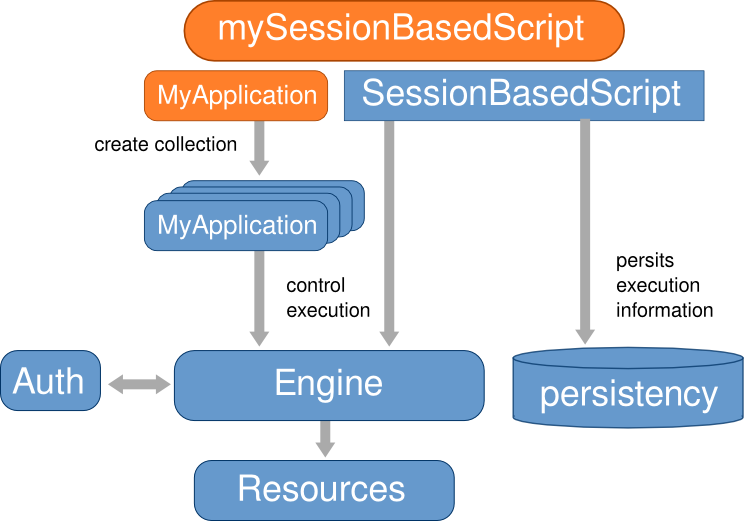
\includegraphics[width=1\textwidth]{fig/GC3Pie_execution_model}
    \column{0.6\textwidth}
  \begin{block}{}
    Each {\color{Blue}resource} has its own access mechanism and thus
    requires its own authentication.
  \end{block}

  \begin{block}{}
    Execution Engine handles the access to computational
    {\color{Blue}resources} transparently.
  \end{block}
  \end{columns}
\end{frame}


\begin{frame}
  \frametitle{GC3Pie Execution model}
  \begin{columns}
    \column{0.5\textwidth}
      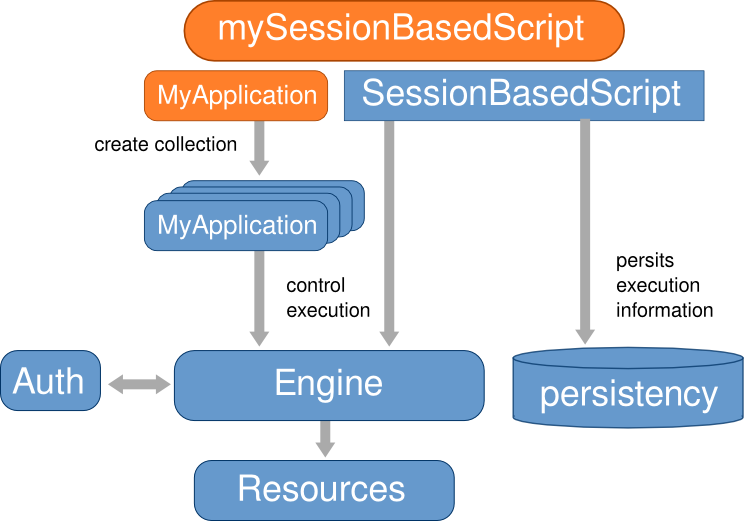
\includegraphics[width=1\textwidth]{fig/GC3Pie_execution_model}
    \column{0.6\textwidth}
  \begin{block}{}
    A convenient {\color{Blue}SessionBasedScript} class contains already
    most of the control logic for instructing the execution engine
  \end{block}

  \begin{block}{}
    \texttt{SessionBasedScript} takes also care of {\color{Blue}persisting}
    execution information
  \end{block}
  \end{columns}
\end{frame}


\begin{frame}
\frametitle{Job dependency management}
  \begin{block}{}
  An \texttt{Engine} manages all jobs concurrently.
  What if there are inter-application dependencies?
  \end{block}

  \begin{block}{}
  GC3Pie provides {\color{Blue}Task composition} support (workflow), created
  programmatically from Python code.
  \end{block}

  \begin{block}{}
  Which means, no graphical editor.  But also means you can create
  workflows {\color{Blue}on-the-fly} as your computation proceeds.
  \end{block}
\end{frame}

\begin{frame}
  \frametitle{References}
  \begin{itemize}
  \item Website: \url{https://code.google.com/p/gc3pie/}
  \item Documentation: \url{http://gc3pie.readthedocs.org/en/latest/}
  \end{itemize}
\begin{center}
Thank you for your attention!
\end{center}
\end{frame}

\end{document}
